%To generate pdf:
%pdflatex description.tex

\documentclass{article}

\usepackage[letterpaper, margin=0.5in, footskip=4ex]{geometry}
\usepackage{xcolor}
\usepackage{graphicx} % Required to insert images
\usepackage{float} % For placing figures EXACTLY where I say
\usepackage{epstopdf}
\usepackage{listings} % Required for insertion of code
\usepackage{amssymb,amsmath}
%%\usepackage[open, openlevel=2]{bookmark}
\usepackage[hidelinks=true,bookmarks=true,bookmarksopen=true]{hyperref}

\graphicspath{ {fig_pdf/} } %If additional directories are needed, place them in additional sets of inner braces e.g {fig_pdf/}{fig_svg/}

\setlength{\parindent}{0pt}
\setlength{\parskip}{1ex}

\begin{document}

\title{Problem Description for Diffusion Through Nanopore}
\author{Tom Pace}
\maketitle

\tableofcontents

%===============================================================================
\section{Background}\label{sec:background}

We study a silica membrane containing nanoscopic circular pores arranged in a two-dimensional lattice.
We desire to understand the rate of transport of different ions through the nanopores,
quantified in terms of an effective diffusion constant.
The pore geometry is variable, as is the diffusion equation governing transport.
The diffusion equation is solved using \texttt{FEniCS}.

%===============================================================================
%not a stand-alone document; intended for inclusion in a larger document

\section{Problem Geometries and Finite Element Meshes}\label{sec:geometry-and-mesh}

%-------------------------------------------------------------------------------
\subsection{Mesoporous Silica Membrane}\label{subsec:silica_membrane}

We study a silica membrane containing nanoscopic circular pores arranged in a two-dimensional lattice.
We desire to understand the rate of transport of different ions through the nanopores,
quantified in terms of an effective diffusion constant.
The pore geometry is variable.

We study both a body-centered rectangular lattice of pores,
as well as a face-centered lattice of pores.
The unit cell geometry has two planes of symmetry.
This symmetry is used to reduce the model to only one quarter of the unit cell.

The body-centered geometry is shown in Figure \ref{fig:body-intro}.
The face-centered geometry is shown in Figure \ref{fig:face-intro}.

\begin{figure}[H]
\centering
\includegraphics[width=1\textwidth]{body-intro.pdf}
\caption{Body-centered geometry}
\label{fig:body-intro}
\end{figure}

\begin{figure}[H]
\centering
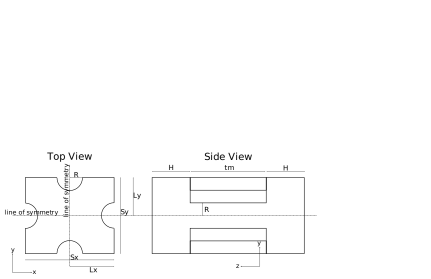
\includegraphics[width=1\textwidth]{face-intro.pdf}
\caption{Face-centered geometry}
\label{fig:face-intro}
\end{figure}

The geometric variables are:

$\begin{array}{rcl}
Sx & = & 2 Lx =\text{Unit cell x-dimension} \\
Sy & = & 2 Ly =\text{Unit cell y-dimension} \\
Lx & = & \frac{Sx}{2} =\text{Model x-dimension} \\
Ly & = & \frac{Sy}{2} =\text{Model y-dimension} \\
R & = & \text{Pore radius} \\
tm & = & \text{Membrane thickness} = \text{Pore length} \\
H & = & \text{Distance from membrane surface to model boundary}
\end{array}$

\texttt{gmsh} is used to generate the finite element mesh.
The mesh is generated from solid geometry defined by its boundary surfaces.
These surfaces, in turn, are defined by their boundaries,
which are defined using points.

\textcolor{red}{\textbf{TODO}}: gmsh geometry (point numbers, etc)

%-------------------------------------------------------------------------------
\subsection{Channel Between Intracellular Membranes}\label{subsec:intracellular_membranes}

We conduct a two-dimensional analysis of the ...

\textcolor{red}{\textbf{TODO}}

\begin{figure}[H]
\centering
\includegraphics[width=0.5\textwidth]{2DProblemGeometry.pdf}
\caption{Channel Geometry}
\label{fig:channel_geometry}
\end{figure}

%-------------------------------------------------------------------------------
\subsection{Zeolites}\label{subsec:zeolites}

\textcolor{red}{\textbf{TODO}}


%===============================================================================
%not a stand-alone document; intended for inclusion in a larger document

\section{Result Calculations}

%-------------------------------------------------------------------------------
\subsection{Effective Diffusion Constant}\label{subsec:D_eff}

To compute the effective diffusion constant,
the three-dimensional diffusion problem is considered from the perspective of a simpler one-dimensional diffusion problem.
Specifically, we wish to consider diffusion in the direction across the membrane.
The Fickian diffusion equation (see Section \ref{sec:unhom_fick}) in one dimension can be written as

\begin{equation}\label{eq:fickslaw_1D}
j = - D_{\mathrm{bulk}} \frac{\mathrm{d}c}{\mathrm{d}s}
\end{equation}

where:

$\begin{array}{rcl}
s & = & \text{position within the one-dimensional domain} \\
j & = & j(s) = \text{flux at any point, in units of number of particles per unit area per unit time} \\
D_{\text{bulk}} & = & \text{diffusion constant of the medium, in units of area per unit time} \\
c & = & c(s) = \text{concentration at any point, in units of number of particles per unit volume} \\
\frac{\mathrm{d}c}{\mathrm{d}s} & = & \text{first spatial derivative of concentration}
\end{array}$

The three-dimensional problem is converted to an equivalent one-dimensional problem
by integrating over the area of the unit cell, in the two directions perpendicular to
the one-dimensional diffusion problem.
The total flux across the membrane will be given by:

\begin{equation}
J_{\mathrm{cell}} = - D_{\mathrm{bulk}}\int_{\mathrm{cell}} \mathrm{d}A\, \frac{\partial c}{\partial s}
\end{equation}

We define the effective diffusion constant such that the integrated flux is the same,
when used with an the average concentration gradient across the membrane:

\begin{equation}\label{eq:Deff_Jcell}
J_{\mathrm{cell}} = - D_{\mathrm{eff}} A_{\mathrm{cell}} \frac{\Delta c}{\Delta s}
\end{equation}

where:

$\begin{array}{rcl}
J_{\text{cell}} & = & \text{integral of flux over the pore, in units of number of particles per unit time} \\
A_{\text{cell}} & = & \text{area of unit cell} \\
D_{\text{eff}} & = & \text{unknown effective diffusion constant} \\
\Delta c & = & \text{change in concentration} \\
\Delta s & = & \text{distance over which concentration changes}
\end{array}$

Re-arranging this equation to solve for the unknown $D_{\mathrm{eff}}$, we have:

\begin{equation}\label{eq:Deff_def}
D_{\mathrm{eff}} = - \frac{J_{\mathrm{cell}}}{A_{\mathrm{cell}}} \frac{\Delta s}{\Delta c}
\end{equation}

The integrated flux, $J_{\mathrm{model}}$, is calculated from the model by integrating
the ion flux over a surface parallel to the membrane surface.
The result should be the same for any such surface capturing the full extents of the model.
That is, the integrated flux should be the same when integrating over the model pore as
when integrating over the upgradient or downgradient boundary of the model.

Specifically, the integrated flux is calculated as:

\begin{equation}
J_{\mathrm{model}} = \int_{\mathrm{model}} \mathrm{d}A\, \left(\hat{n} \cdot \vec{j} \right)
 = - D_{\mathrm{bulk}} \int_{\mathrm{model}} \mathrm{d}A\, \left(\hat{n} \cdot \vec{\nabla} c \right)
\end{equation}

where $\hat{n}$ is the directed normal to the surface,
and $c$ is the concentration field found by solving the model.

Because of the use of planes of symmetry (see Section \ref{subsec:geometry}),
the flux obtained by integration is only one quarter of the total for the unit cell.
That is, $J_{\mathrm{cell}} = 4 J_{\mathrm{model}}$.
With $A_{\mathrm{cell}} = 4 Lx Ly$, we have:

\begin{equation}
D_{\mathrm{eff}} = - \frac{4 J_{\mathrm{model}}}{4 Lx Ly} \frac{\Delta s}{\Delta c}
 = - \frac{J_{\mathrm{model}}}{Lx Ly} \frac{\Delta s}{\Delta c}
\end{equation}

For convenience, we define the integral

\begin{equation}
I_{\mathrm{gc}} = \int_{\mathrm{model}} \mathrm{d}A\, \left(\hat{n} \cdot \vec{\nabla} c \right)
\end{equation}

then the flux integral is simply

\begin{equation}
J_{\mathrm{model}} = - D_{\mathrm{bulk}} I_\mathrm{gc}
\end{equation}

and the effective diffusion constant is

\begin{equation}
D_{\mathrm{eff}} = D_{\mathrm{bulk}} \frac{I_\mathrm{gc}}{Lx Ly} \frac{\Delta s}{\Delta c}
\end{equation}

This can also be written as

\begin{equation}
\frac{D_{\mathrm{eff}}}{D_{\mathrm{bulk}}} = \frac{I_\mathrm{gc}}{Lx Ly} \frac{\Delta s}{\Delta c}
\end{equation}

The values of $\Delta c$ and $\Delta s$ are calculated by extracting
the concentration result at two points located symmetrically on opposite sides of the membrane.
The difference in concentration between these two points is $\Delta c$,
and the distance between them is $\Delta s$.

Slightly different results for the value of $D_{\mathrm{eff}}$ could be attained by selecting different
pairs of symmetrically located points.
For consistency, the results here are taken with these two points located
along the centerline of the pore, at both faces of the membrane.

%-------------------------------------------------------------------------------
\subsection{Free Volume Fraction}\label{subsec:volfrac}

The free volume fraction, $\phi$ is defined here as

\begin{equation}
\phi = \frac{\text{pore area}}{\text{unit cell area}}
= \frac{\pi R^2}{Sx Sy} = \frac{\pi R^2}{4 Lx Ly}
\end{equation}



%===============================================================================
%not a stand-alone document; intended for inclusion in a larger document

\subsection{Unhomogenized Fickian Diffusion Equation}\label{subsec:unhom_fick}

\subsubsection{Governing Differential Equation}\label{subsubsec:unhom_fick_gov}
For particle flux defined as 

\begin{equation}
\vec{j} = - D_{\mathrm{bulk}} \vec{\nabla} c
\end{equation}

The Fickian diffusion equation can be written:
\begin{equation}
\frac{\partial c}{\partial t} = - \vec{\nabla} \cdot \vec{j}
\end{equation}

where:

$\begin{array}{rcl}
c & = & c(x,y,z) = \text{the particle concentration field (number of particles per unit volume)} \\
t & = & \text{time} \\
\vec{j} & = & \vec{j}(x,y,z) = \text{the particle flux field (number of particles per unit area per unit time)} \\
D & = & \text{the implicit diffusion constant of the solvent (unit area per unit time)}
\end{array}$

For constant $D_{\mathrm{bulk}}$, this can be written as

\begin{equation}
\frac{\partial c}{\partial t} = D_{\mathrm{bulk}} \nabla^2 c
\end{equation}

We seek the solution at equilibrium, defined by
$\frac{\partial c}{\partial t} = 0$ at all points in the problem domain.
Thus, we seek to solve

\begin{equation}
D_{\mathrm{bulk}} \nabla^2 c = 0
\end{equation}

subject to boundary conditions.

Assuming $D_{\mathrm{bulk}}$ is any nonzero constant, this is clearly the same as

\begin{equation}
\nabla^2 c = 0
\end{equation}

\subsubsection{Weak Form}\label{subsubsec:unhom_fick_weak}

For solution in \texttt{FEniCS}, a weak form of this equation is required.
Multiplying by a test function $v$ and integrating over the problem domain,

\begin{equation}
\int_{\Omega} \left(\nabla^2 c \right) v \,\mathrm{d}^3x = 0
\end{equation}

Using the product rule
\begin{equation}
\vec{\nabla} \cdot \left( v \vec{\nabla} c \right) =
v \left(\vec{\nabla} \cdot \vec{\nabla} c \right) + \vec{\nabla}c \cdot \vec{\nabla}v =
v \left(\nabla^2 c \right) + \vec{\nabla}c \cdot \vec{\nabla}v
\end{equation}

\begin{equation}
\left(\nabla^2 c \right) v =
\vec{\nabla} \cdot \left( v \vec{\nabla} c \right) - \vec{\nabla}c \cdot \vec{\nabla}v
\end{equation}

to integrate by parts, the equation becomes
\begin{equation}
\int_{\Omega} \left(\nabla^2 c \right) v \,\mathrm{d}^3x =
\int_{\Omega} \vec{\nabla} \cdot \left( v \vec{\nabla} c \right) \,\mathrm{d}^3x
- \int_{\Omega} \left( \vec{\nabla}c \cdot \vec{\nabla}v \right) \,\mathrm{d}^3x =0
\end{equation}

Applying the divergence theorem (Gauss's theorem):
\begin{equation}
\int_{\partial\Omega} \left( \hat{n} \cdot \vec{\nabla} c \right) v\,\mathrm{d}s
- \int_{\Omega} \left( \vec{\nabla}c \cdot \vec{\nabla}v \right) \,\mathrm{d}^3x = 0
\end{equation}

\begin{equation}
\int_{\Omega} \left( \vec{\nabla}c \cdot \vec{\nabla}v \right) \,\mathrm{d}^3x =
\int_{\partial\Omega} \left( \hat{n} \cdot \vec{\nabla} c \right) v\,\mathrm{d}s
\end{equation}

In this case, we have both Dirichlet and von Neumann boundary conditions:
there are some boundary surfaces where the concentration is known,
and others where the particle flux is known.
Specifically, known concentrations are applied at both the top and bottom of the model,
and the particle flux must be zero for all other boundary surfaces.
Defining $\Gamma_D$ as the Dirichlet boundary surfaces,
and $\Gamma_N$ as the von Neumann boundary surfaces, we obtain

\begin{equation}
\int_{\Omega} \left( \vec{\nabla}c \cdot \vec{\nabla}v \right) \,\mathrm{d}^3x =
\int_{\Gamma_D} \left( \hat{n} \cdot \vec{\nabla} c \right) v\,\mathrm{d}s
+\int_{\Gamma_N} \left( \hat{n} \cdot \vec{\nabla} c \right) v\,\mathrm{d}s
\end{equation}

For the Dirichlet boundary surfaces (where the concentration is known),
the test function $v$ must be equal to zero,
as the variation of the unknown function must be zero at points where the function is known.

Furthermore, a flux of zero requires that the derivative of the concentration in a direction
normal to the boundary surface is zero.
That is, $\hat{n} \cdot \vec{\nabla} c = 0$ at all points on the von Neumann boundaries.

Therefore, the governing equation is simply
\begin{equation}
\int_{\Omega} \left( \vec{\nabla}c \cdot \vec{\nabla}v \right) \,\mathrm{d}^3x = 0
\end{equation}

In terms of \texttt{FEniCS}, this means that the bilinear form is
$a(c,v)=\left( \vec{\nabla}c \cdot \vec{\nabla}v \right) \,\mathrm{d}^3x$,
and the linear form is constant, zero.

\subsubsection{Expected Results}\label{subsubsec:unhom_fick_expected}

The effective diffusion constant of Section \ref{subsec:D_eff}
was derived by simplification of the governing equation
to an unhomogenized Fickian diffusion equation.
Consequently, the effective diffusion constant for this equation
can be estimated very simply.

In the absence of surface chemistry phenomena,
we should expect the concentration gradient
to be essentially constant within the pore, and oriented only in the axial direction.
That is, the concentration profile within the pore will be linear,
and at any cross-section there is only a single value of the concentration.
This implies that the problem is very nearly one-dimensional,
as assumed in the definition of $D_{\mathrm{eff}}$.

Defining the concentration gradient within the pore as
\begin{equation}
\vec{\nabla} c = \left(\frac{\mathrm{d}c}{\mathrm{d}s}\right)_{\mathrm{pore}} \hat{n}
\end{equation}

where $\left(\frac{\mathrm{d}c}{\mathrm{d}s}\right)_{\mathrm{pore}}$ is a constant,
the integrated flux within the pore is

\begin{equation}
J_\mathrm{cell} = -D_\mathrm{bulk} \int_\mathrm{cell} \mathrm{d}A\, \left(\frac{\mathrm{d}c}{\mathrm{d}s}\right)_{\mathrm{pore}}
 = -D_\mathrm{bulk} A_\mathrm{pore} \left(\frac{\mathrm{d}c}{\mathrm{d}s}\right)_{\mathrm{pore}}
\end{equation}

Note that the area in this formula is the area of the pore only,
rather than the entire unit cell, because only the pore is within the problem domain
at a cross-section through the pore.

From equation \ref{eq:Deff_Jcell}, we have

\begin{equation}
J_{\mathrm{cell}} = - D_{\mathrm{eff}} A_{\mathrm{cell}} \frac{\Delta c}{\Delta s}
\end{equation}

But with a constant concentration gradient,

\begin{equation}
\frac{\Delta c}{\Delta s} = \left(\frac{\mathrm{d}c}{\mathrm{d}s}\right)_{\mathrm{pore}}
\end{equation}

So,

\begin{equation}
J_{\mathrm{cell}} = - D_{\mathrm{eff}} A_{\mathrm{cell}} \left(\frac{\mathrm{d}c}{\mathrm{d}s}\right)_{\mathrm{pore}}
 = -D_\mathrm{bulk} A_\mathrm{pore} \left(\frac{\mathrm{d}c}{\mathrm{d}s}\right)_{\mathrm{pore}}
\end{equation}

This simplifies to

\begin{equation}
\frac{D_\mathrm{eff}}{D_\mathrm{bulk}} = \frac{A_\mathrm{pore}}{A_\mathrm{cell}}
\end{equation}

which matches the definition of the free volume fraction from Section \ref{subsec:volfrac}, so

\begin{equation}
\frac{D_\mathrm{eff}}{D_\mathrm{bulk}} = \phi
\end{equation}

for unhomogenized Fickian diffusion.


%===============================================================================
%not a stand-alone document; intended for inclusion in a larger document

\section{Unhomogenized Smoluchowski Equation}\label{sec:unhom_smol}

%-------------------------------------------------------------------------------
\subsection{Governing Differential Equation}\label{subsec:unhom_smol_gov}

\textcolor{red}{\textbf{TODO}}: need reference for Smoluchowski equation

For an environment free of particle sources and sinks,
the diffusion equation can still be written as:
\begin{equation}
  \frac{\partial c}{\partial t} = - \vec{\nabla} \cdot \vec{j}
\end{equation}

but for the Smoluchowski equation, the particle flux is defined as

\begin{equation}
  \vec{j} = - D_{\mathrm{bulk}} e^{-\beta \psi} \vec{\nabla} \left( e^{\beta \psi} c \right)
\end{equation}

where:

$\begin{array}{rcl}
c & = & c(x,y,z) = \text{the particle concentration field (number of particles per unit volume)} \\
t & = & \text{time} \\
\vec{j} & = & \vec{j}(x,y,z) = \text{the particle flux field (number of particles per unit area per unit time)} \\
D_{\mathrm{bulk}} & = & \text{the implicit diffusion constant of the solvent (unit area per unit time)} \\
\psi & = & \psi(x,y,z) = \text{the potential field} \\
\beta & = & 1/k_B T
\end{array}$

Combining these equations, the governing equation for steady-state conditions ($\frac{\partial c}{\partial t} = 0$) is

\begin{equation}
  \vec{\nabla} \cdot \left( D_{\mathrm{bulk}} e^{-\beta \psi} \vec{\nabla} \left( c e^{\beta \psi} \right) \right) = 0
\end{equation}

\textcolor{red}{\textbf{TODO}}: need reference for Slotboom transformation

The mathematics are simplified considerably by making use of the Slotboom transformation:

\begin{equation}\label{eq:SlotboomTrans}
  \begin{array}{rcl}
    \overline{D} & = & D_{\mathrm{bulk}} e^{-\beta \psi} \\
    \overline{c} & = & c e^{\beta \psi}
  \end{array}
\end{equation}

which results in the governing equation

\begin{equation}
  \vec{\nabla} \cdot \left( \overline{D} \vec{\nabla} \left( \overline{c} \right) \right) = 0
\end{equation}

Applying the appropriate product rule for the divergence operator in this case,

\begin{equation}\label{eq:SmolSlotboomDiff}
  \boxed{
    \overline{D} \nabla^2 \overline{c} + \left( \vec{\nabla} \overline{c} \right) \cdot \left( \vec{\nabla} \overline{D} \right) = 0
  }
\end{equation}

For the diffusion of ions in an electrostatic field, the potential field is given by

\begin{equation}
  \psi=q \Phi
\end{equation}

where:

$\begin{array}{rcl}
q & = & \text{the electric charge of the ion species} \\
\Phi & = & \text{the electric potential field}
\end{array}$

This means that the Slotboom transformation (Equation \ref{eq:SlotboomTrans}) can be written as

\begin{equation}\label{eq:SlotboomTransWithQ}
  \begin{array}{rcl}
    \overline{D} & = & D_{\mathrm{bulk}} e^{-\beta q \Phi} \\
    \overline{c} & = & c e^{\beta q \Phi}
  \end{array}
\end{equation}

Note that the applied boundary conditions must be transformed as well.
This is straightforward for Dirichlet boundary conditions,
as Equation \ref{eq:SlotboomTransWithQ} can be applied directly
to obtain the Dirchlet value of $\overline{c}$ from that of $c$.
Neumann boundary conditions, however, are more complicated.
We wish to specify a value of $\frac{\partial c}{\partial n} = \vec{\nabla} c \cdot \hat{n}$,
but solving the transformed equation requires converting this to specification of the value
$\frac{\partial \overline{c}}{\partial n} = \vec{\nabla} \overline{c} \cdot \hat{n}$.

\begin{equation}\begin{array}{rcl}
  \frac{\partial \overline{c}}{\partial n} & = & \vec{\nabla} \overline{c} \cdot \hat{n} \\
  & = & \vec{\nabla} \left( c e^{\beta q \Phi} \right) \cdot \hat{n} \\
  & = & \left( c \vec{\nabla} e^{\beta q \Phi} +  e^{\beta q \Phi} \vec{\nabla} c \right) \cdot \hat{n} \\
  & = & c \vec{\nabla} \left(e^{\beta q \Phi} \right) \cdot \hat{n}
  + e^{\beta q \Phi} \vec{\nabla} \left( c \right) \cdot \hat{n} \\
  & = & c \beta q e^{\beta q \Phi} \vec{\nabla} \left( \Phi \right) \cdot \hat{n}
  + e^{\beta q \Phi} \vec{\nabla} \left( c \right) \cdot \hat{n} \\
  & = & c \beta q e^{\beta q \Phi} \frac{\partial \Phi}{\partial n}
  + e^{\beta q \Phi} \frac{\partial c}{\partial n} \\
  \frac{\partial \overline{c}}{\partial n} & = & e^{\beta q \Phi}
  \left( c \beta q \frac{\partial \Phi}{\partial n} + \frac{\partial c}{\partial n} \right)
\end{array}\end{equation}

Thus, the Neumann boundary conditions on $\overline{c}$ depend not only on
those of $c$, but also on the potential field and its normal derivative at the boundary.
In the case of this model, the normal derivative of $c$ is specified to be zero
at all Neumann boundaries, as is the normal derivative of $\Phi$.
Thus, the boundary condition on $\overline{c}$ is also that its normal derivative is zero
at the Neumann boundaries.

Finally, after solution of the transformed equation,
the ionic concentration field is calculated from the inverse transformation,

\begin{equation}
  c = \overline{c} e^{-\beta \psi} = \overline{c} e^{-\beta q \Phi}
\end{equation}

%-------------------------------------------------------------------------------
\subsection{Weak Form}\label{subsec:unhom_smol_weak}

Starting from the governing differential equation (Equation \ref{eq:SmolSlotboomDiff}),
multiplying by a test function $v$ and integrating over the problem domain, we have

\begin{equation}\label{eq:SmolWeakStart}
  \int_{\Omega} \overline{D} v \left( \nabla^2 \overline{c} \right) \,\mathrm{d}^3x 
  + \int_{\Omega} v \left( \vec{\nabla} \overline{c} \right) \cdot \left( \vec{\nabla} \overline{D} \right) \,\mathrm{d}^3x = 0
\end{equation}

Using the same product rule as Equation \ref{eq:product_rule_divergence}, 
we have

\begin{equation}
  \vec{\nabla} \cdot \left( \overline{D} v \vec{\nabla} \overline{c} \right) =
  \overline{D} v \left(\vec{\nabla} \cdot \vec{\nabla} \overline{c} \right)
  + \vec{\nabla}\overline{c} \cdot \vec{\nabla} \left( \overline{D} v \right) =
  \overline{D} v \left(\nabla^2 \overline{c} \right)
  + \vec{\nabla}\overline{c} \cdot \vec{\nabla} \left( \overline{D} v \right)
\end{equation}

And so, applying the product rule for the gradient of two scalars,
\begin{equation}
  \overline{D} v \left(\nabla^2 \overline{c} \right) =
  \vec{\nabla} \cdot \left( \overline{D} v \vec{\nabla} \overline{c} \right)
  - \vec{\nabla}\overline{c} \cdot \left( \overline{D} \vec{\nabla} v + v \vec{\nabla} \overline{D} \right)
\end{equation}

\begin{equation}
  \overline{D} v \left(\nabla^2 \overline{c} \right) =
  \vec{\nabla} \cdot \left( \overline{D} v \vec{\nabla} \overline{c} \right)
  - \overline{D} \left(\vec{\nabla}\overline{c}\right) \cdot \left(\vec{\nabla}v\right)
  - v \left(\vec{\nabla}\overline{c}\right) \cdot \left(\vec{\nabla}\overline{D}\right)
\end{equation}

Taking the integral over the problem domain, this gives us

\begin{equation}
  \int_{\Omega} \overline{D} v \left(\nabla^2 \overline{c} \right) \,\mathrm{d}^3x=
  \int_{\Omega} \vec{\nabla} \cdot \left( \overline{D} v \vec{\nabla} \overline{c} \right) \,\mathrm{d}^3x
  - \int_{\Omega} \overline{D} \left(\vec{\nabla}\overline{c}\right) \cdot \left(\vec{\nabla}v\right)\,\mathrm{d}^3x
  - \int_{\Omega} v \left(\vec{\nabla}\overline{c}\right) \cdot \left(\vec{\nabla}\overline{D}\right) \,\mathrm{d}^3x
\end{equation}

Substituting this into Equation \ref{eq:SmolWeakStart},
the governing equation becomes

\begin{equation}
  \int_{\Omega} \vec{\nabla} \cdot \left( \overline{D} v \vec{\nabla} \overline{c} \right) \,\mathrm{d}^3x
  - \int_{\Omega} \overline{D} \left(\vec{\nabla}\overline{c}\right) \cdot \left(\vec{\nabla}v\right)\,\mathrm{d}^3x
  - \int_{\Omega} v \left(\vec{\nabla}\overline{c}\right) \cdot \left(\vec{\nabla}\overline{D}\right) \,\mathrm{d}^3x
  + \int_{\Omega} v \left( \vec{\nabla} \overline{c} \right) \cdot \left( \vec{\nabla} \overline{D} \right) \,\mathrm{d}^3x = 0
\end{equation}

The final two terms cancel one another.
Using the divergence theorem (Gauss's theorem), the result is
\begin{equation}
  \int_{\partial\Omega} \overline{D} v \left(\hat{n} \cdot \vec{\nabla}\overline{c}\right) \,\mathrm{d}s
  - \int_{\Omega} \overline{D} \left(\vec{\nabla}\overline{c}\right) \cdot \left(\vec{\nabla}v\right)\,\mathrm{d}^3x
  = 0
\end{equation}

The boundary term separates into the Dirichlet boundaries (where $\overline{c}$ is known and therefore $v=0$),
and the Neumann boundaries, as discussed in Section \ref{subsec:unhom_smol_gov},
where it was noted that $\hat{n} \cdot \vec{\nabla} \overline{c} = 0$ at all points on the von Neumann boundaries.
Thus, the boundary term is zero in its entirety,
and so the weak form of the transformed Smoluchowski equation in this case is

\begin{equation}
  \int_{\Omega} \overline{D} \left(\vec{\nabla}\overline{c}\right) \cdot \left(\vec{\nabla}v\right)\,\mathrm{d}^3x = 0
\end{equation}

In terms of \texttt{FEniCS}, this means that the bilinear form is

\begin{equation}
  \boxed{
    a(\overline{c},v)= \overline{D} \left(\vec{\nabla}\overline{c}\right) \cdot \left(\vec{\nabla}v\right)\,\mathrm{d}^3x
  }
\end{equation}

and the linear form is constant, zero, provided there are no nonzero Neumann conditions.


%-------------------------------------------------------------------------------
\subsection{Applied Potential}\label{subsec:unhom_smol_potential}

To solve the Smoluchowski diffusion equation, the electric potential $\Phi$ must be given.
Here, we will calculate the electric potential using the linearized Poisson-Boltzmann equation
(Equation 15-29 in \cite{McQuarrie-StatMech}).

\begin{equation}\label{eq:PoissonBoltzmann}
  \nabla^2 \Phi = \kappa^2 \Phi
\end{equation}

where the constant $\kappa$ has dimensions of inverse length.
It is also noted in \cite{McQuarrie-StatMech} that this equation becomes exact
in the limit $\kappa \rightarrow 0$,
which corresponds to very low ionic concentrations.

The length $\lambda_D = 1/\kappa$ is commonly known as the Debye length.
A formula for the calculation of $\kappa^2$ is provided in \cite{McQuarrie-StatMech},
but it requires knowing the spatial distribution of the ions.
Instead, we will use the Debye length as a property of the problem domain.
Then, with appropriate boundary conditions,
the electric potential can be found by Finite Element solution of Equation \ref{eq:PoissonBoltzmann}.

\textcolor{red}{\textbf{TODO}}: show sketch of electrostatic boundary conditions

To solve for the potential in \texttt{FEniCS},
a weak form of the Poisson-Boltzmann equation (Equation \ref{eq:PoissonBoltzmann}) is required.
Multiplying by the test function $v$ and integrating over the problem domain, we obtain

\begin{equation}
  \int_{\Omega} \left(\nabla^2 \Phi \right) v \,\mathrm{d}^3x = \frac{1}{\lambda_D^2} \int_{\Omega} \Phi v \,\mathrm{d}^3x
\end{equation}

Using the same product rule as Equation \ref{eq:product_rule_divergence} for integration by parts, this becomes
\begin{equation}
  \int_{\Omega} \vec{\nabla} \cdot \left( v \vec{\nabla} \Phi \right) \,\mathrm{d}^3x
  - \int_{\Omega} \vec{\nabla}\Phi \cdot \vec{\nabla}v \,\mathrm{d}^3x
  = \frac{1}{\lambda_D^2} \int_{\Omega} \Phi v \,\mathrm{d}^3x
\end{equation}

Applying the divergence theorem (Gauss's theorem),
\begin{equation}
  \int_{\partial\Omega} \left( \hat{n} \cdot \vec{\nabla} \Phi \right) v \,\mathrm{d}s
  - \int_{\Omega} \vec{\nabla}\Phi \cdot \vec{\nabla}v \,\mathrm{d}^3x
  = \frac{1}{\lambda_D^2} \int_{\Omega} \Phi v \,\mathrm{d}^3x
\end{equation}

The boundary term separates into the Dirichlet boundaries (where $\Phi$ is known and therefore $v=0$),
and the Neumann boundaries, which in this case will have zero electric field normal to the surface.
This condition requires that the derivative of the potential normal to the surface is zero,
and so $\hat{n} \cdot \vec{\nabla} \Phi = 0$ at all points on the von Neumann boundaries.
Thus, the boundary term is zero in its entirety, and the equation becomes

\begin{equation}
  \frac{1}{\lambda_D^2} \int_{\Omega} \Phi v \,\mathrm{d}^3x
  + \int_{\Omega} \vec{\nabla}\Phi \cdot \vec{\nabla}v \,\mathrm{d}^3x
  = 0
\end{equation}

In terms of \texttt{FEniCS}, this means that the bilinear form is

\begin{equation}
  \boxed{
    a(\Phi,v)=\left(\frac{1}{\lambda_D^2} \Phi v  + \vec{\nabla}\Phi \cdot \vec{\nabla}v \right) \,\mathrm{d}^3x
  }
\end{equation}

and the linear form is constant, zero, provided there are no nonzero Neumann conditions.

%-------------------------------------------------------------------------------
\subsection{Expected Results}\label{subsec:unhom_smol_expected}

The Smoluchowski diffusion equation does not model any interaction between the ions themselves.
Therefore, with an applied potential of zero,
the solution should be the same as for the
unhomogenized Fickian diffusion equation (Section \ref{subsec:unhom_fick_expected}).

%-------------------------------------------------------------------------------
\subsection{Results from Unhomogenized Smoluchowski Equation}\label{subsec:res_unhom_smol}

\textcolor{red}{\textbf{TODO}}

\begin{figure}[H]
\centering
\maybeincludegraphics[width=1\textwidth]{../data/postproc/thin-shot/ratio_vs_phi.pdf}
\caption{Result of Smoluchowski Diffusion Analysis}
\label{fig:uh_smol_D_vs_phi}
\end{figure}


%-------------------------------------------------------------------------------
\section{Homogenized Fickian Diffusion Equation}\label{sec:hom_fick}

\textcolor{red}{\textbf{TODO}}


\end{document}
